
\chapter{Financial Derivatives and Pricing}

The machinery of stochastic processes and stochastic calculus developed in the previous chapters finds its most celebrated application in the theory of \emph{financial derivatives}.
The problem it solves is easy to state and was, for most of a century, believed to have no objective answer: what is the \emph{fair price} of a contract whose value depends on the unknown future price of something else?
This chapter builds the answer from the ground up.
We first describe the structure of financial markets and the main asset classes; we then introduce options and the no-arbitrage principle; and we finally derive the Black--Scholes equation and solve it, obtaining the formula that in 1973 turned derivative pricing from an art into a science.


\section{Financial markets}

A \emph{financial market} is a physical or virtual venue in which agents exchange \emph{assets} at a \emph{spot price} (instantaneous price) $S(t)$, determined by the law of supply and demand.
The participants are heterogeneous --- banks, hedge funds, brokers, individual traders --- and so are the venues.
\emph{Stock markets} in particular come in three flavours: the \emph{official exchanges} (NYSE, LSE, \ldots), of which there are about $200$ worldwide, historically paper-based; the fully \emph{electronic} exchanges (Nasdaq, Euronext, \ldots), where trading is algorithmic; and \emph{hybrid} venues such as today's NYSE, which combine both.
Alongside the official markets there exist non-official ones, distinguished by the absence of intermediaries.

% CLAUDE NOTE: the following two paragraphs of background for readers new to finance
% were added at the author's request (2026-07-06); they expand the prose without
% altering any of the notes' content.
Since this book is written for physicists, it is worth pausing on how a trade actually happens, because the microscopic mechanism is what gives the spot price its meaning.
At any instant, an exchange maintains for each asset an \emph{order book}: a list of offers to buy at stated prices (the \emph{bids}) and offers to sell at stated prices (the \emph{asks}).
The highest bid and the lowest ask face each other across a small gap, the \emph{bid--ask spread}; a trade occurs when someone accepts the best price on the opposite side, and the price at which this happens is the quoted price of the asset.
The market is called \emph{liquid} when the book is thick --- when there are so many standing offers that one can buy or sell a large quantity at any moment without moving the price appreciably.
Liquidity is the market's analogue of a good thermal bath: it is what allows a single agent to exchange with the collective without perturbing it, and most of the idealizations of this chapter (continuous trading, negligible spread) are statements about high liquidity.

Two more pieces of jargon will recur.
An investor is \emph{long} an asset after buying it, profiting if the price rises; and is \emph{short} after selling an asset it does not own --- borrowing it, selling it, and planning to buy it back later --- profiting if the price falls.
Short selling looks exotic but is essential: it is what allows negative positions, and therefore hedges, to exist; we will meet a short position at the heart of the Black--Scholes argument.

The central object of the theory is the spot price, and two of its properties deserve to be stated explicitly.
First, the spot price is \emph{unique}: at any given time there is a single price in the whole market --- there is no ``price here'' and ``price there''.
(Why this is so is a question we defer for a few pages; the answer is arbitrage.)
Second, it is a price of \emph{equilibrium}: it arises from the matching of supply and demand, i.e.\ from the meeting of the best ask and the best bid, with a bid--ask spread $\Delta(\text{ask},\,\text{bid})\to 0$.
In reality $\Delta>0$, because of transaction costs and related frictions, but the idealization is a good one for liquid markets.

Under what conditions does such an equilibrium price exist at all?
The classical answer requires the market to be \emph{atomistic} --- no single agent has a large influence --- and to satisfy three structural conditions.
There must be \emph{perfect competition and information}: entry and exit are free, and all participants know everything, instantly.
There must be \emph{no arbitrage}: no free profits exist, and any asymmetry of information is resolved immediately.
And the market must be \emph{complete}: the assets already present span the entire space of probabilities, so that the payoff of any new asset can be replicated with existing ones.
When these conditions hold, the \emph{Arrow--Debreu} model applies, and one can prove that a system of equilibrium prices exists.
In such a market the gain available to an investor is the \emph{interest rate}, plus a premium for bearing \emph{risk} --- a decomposition that will guide us throughout this chapter.


\section{Risk and the Efficient Market Hypothesis}

\subsection{Types of risk}

Since risk is what one is paid to bear, we should say what kinds there are.
Financial risk is traditionally classified into three categories.
\emph{Operational risk} covers human errors, computer crashes, and similar accidents of implementation --- a category whose weight has grown with automation: today some $60$--$75\%$ of all transactions worldwide are executed by algorithmic trading, much of it speculative high-frequency trading.
% CLAUDE NOTE: the algorithmic-trading figure is from the course slides
% (Mercati & Strumenti Finanziari), added 2026-07-06.
\emph{Credit risk} is the risk that the counterparty does not honour the obligations of the contract --- the risk of insolvency.
\emph{Market risk}, finally, is the one that will concern us: the random fluctuation of prices themselves, caused partly by the internal dynamics of supply and demand, partly by exogenous factors (politics, disasters, \ldots), and partly by psychological factors --- imitation, panic --- whose study belongs to \emph{behavioural economics}.
The Black--Scholes theory we develop below deals with market risk only; credit risk is assumed away, an assumption whose limits became painfully visible in 2008.

\subsection{The Efficient Market Hypothesis}

The fundamental question, on which the applicability of everything we have built so far depends, is this:

\medskip
\begin{center}
\emph{Is the dynamics of an asset a Markov process?}
\end{center}
\medskip

Figure~\ref{fig:djia} shows why the question is not rhetorical: the trajectory of a major index looks like the noisy paths of the previous chapters, but it visibly responds to identifiable exogenous shocks --- trade disputes, a pandemic, central-bank decisions --- and one may legitimately ask whether such a history can be modelled by a memoryless It\^o SDE driven by market risk alone.

% Figure after the course slides (Mercati & Strumenti Finanziari);
% generated by images/code_for_images/djia_events.py from FRED series DJIA.
\begin{figure}[h!]
\centering
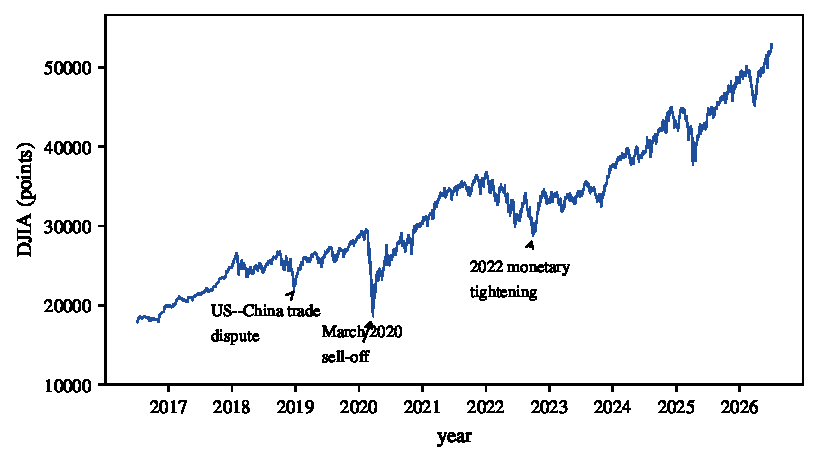
\includegraphics[width=0.9\textwidth]{images/djia_events.pdf}
\caption{The Dow Jones Industrial Average, daily closes 2016--2026 (FRED series DJIA), with some major exogenous events annotated. The fundamental question of this section: can this dynamics be modelled as a Markov process? Generated by \texttt{images/code\_for\_images/djia\_events.py}.}
\label{fig:djia}
\end{figure}

If prices carry memory, the Fokker--Planck machinery of Chapter~3 does not apply, and neither do the SDE models of Chapter~4.
The Markov property holds only if the \emph{Efficient Market Hypothesis} (EMH) does.
The EMH, formulated by Fama in 1970\cite{Fama1970}, states that the market reflects fully and instantaneously all available information: whatever can be known about an asset is already incorporated in its current price.
If this is true, the past adds nothing to the present --- which is precisely the Markov property.
The hypothesis carries several implications: information must be instantly and freely available to all agents (only the present matters); the market must be \emph{liquid}, so that anyone can buy and sell easily; and transaction costs must be negligible.
Assembling the pieces, we can summarize the structural assumptions of this chapter in a single line:
\begin{equation}
\text{EMH} + \text{no arbitrage} + \text{completeness} \;=\; \text{Arrow--Debreu}.
\end{equation}
The EMH is the hypothesis that mathematical finance later made rigorous in the fundamental theorems of asset pricing (Section~\ref{sec:rn-girsanov}); and if the market is efficient, the economically rational standard model for asset prices is Samuelson's geometric Brownian motion --- work recognized with the 1970 Nobel Prize in Economics.
% CLAUDE NOTE: the FTAP remark and the Samuelson Nobel mention follow the course slides
% (Mercati & Strumenti Finanziari), added 2026-07-06.
Whether real markets satisfy the EMH is an empirical question --- and the answer, as we shall see in Section~\ref{sec:gbm-limits} and again in Chapter~7, is ``only approximately''.


\section{Financial assets}

Before specializing to derivatives, it is worth surveying what is actually traded.
The main asset classes are the following.
\begin{itemize}
    \item \textbf{Currencies}: money itself, traded against other money.
    \item \textbf{Commodities}: energy, precious metals, agricultural products, and so on.
    \item \textbf{Stocks} (equities): securities issued by a company to raise capital by selling a fraction of its ownership, without any obligation of repayment.
    For the buyer they offer visibility, a voice in company decisions, and possible dividends.
    A \emph{stock index} is the average (arithmetic or weighted) value of a group of equity titles --- the S\&P\,500, which averages five hundred large American companies weighted by capitalization, will reappear several times in this book; other examples are the Dow Jones (USA), the FTSE\,100 (UK), the CAC\,40 (France), the DAX (Germany), the FTSE\,MIB (Italy), and the Nikkei (Japan).
    % CLAUDE NOTE: index examples from the course slides, added 2026-07-06.
    \item \textbf{Bonds} (obligations): debt securities issued by states or companies to raise large sums; they have a \emph{maturity} $T$ at which the capital is repaid with interest, and are comparatively low-risk.
    They are the subject of Chapter~6.
    \item \textbf{Derivatives}: contracts whose value derives from other assets --- the subject of the present chapter.
    \item \textbf{Cryptocurrencies}: assets living outside the official markets.
\end{itemize}
Portfolios mixing these classes (gold, currencies, stocks, bonds, ETFs\ldots) are the standard tool of diversification and, in general, of speculation.
A \emph{portfolio} is simply a weighted collection of assets held together, and \emph{diversification} --- not putting all the eggs in one basket --- has a rationale a physicist will recognize at once: if the fluctuations of $N$ assets were independent, the relative fluctuation of their sum would shrink as $1/\sqrt{N}$, exactly like the relative energy fluctuations of $N$ weakly coupled subsystems.
Mixing imperfectly correlated assets therefore reduces risk at no cost in average return; the catch, to which we return in Chapter~7, is that in a crisis the correlations rise and the $\sqrt{N}$ protection evaporates precisely when it is needed.
% CLAUDE NOTE: the diversification paragraph was added for readers new to finance at the
% author's request (2026-07-06).
To appreciate the scale of all this: the total value of global financial assets is approximately \$461 trillion, against a world GDP of roughly \$100 trillion.
Finance is not a small correction to the real economy; by market value it is several times larger.


\section{Derivatives and options}

A \emph{derivative} is a contract between a buyer and a seller whose value \emph{derives} from the value of other financial instruments (currencies, stocks, etc.).
The idea is old: derivatives appeared in the Netherlands in the 1600s for the tulip trade, and the first recorded example is usually attributed to Aristotle (\emph{Politics} I.xi), where Thales, expecting a good olive harvest, secured in advance the right to use the local olive presses.
Then as now, derivatives serve two purposes: \emph{hedging}, i.e.\ insurance against unfavourable price movements, and \emph{speculation}, i.e.\ profiting from anticipated ones.

One important type of derivative is the (\emph{stock}) \textbf{option}.
An option is a contract between two parties --- the \textbf{writer}, who sells the contract, and the \textbf{holder}, who buys it --- granting the holder the right, but not the obligation, to buy (\textbf{call}) or sell (\textbf{put}) from/to the writer the \emph{underlying asset} (the stock) at a fixed price $X$, the \emph{strike}, at a future time $T$, the \emph{maturity}.

The contract is fundamentally \emph{asymmetric}, and the asymmetry is what makes pricing non-trivial.
The holder may exercise the option or walk away, at will; the writer, if the holder exercises, \emph{must} sell (or buy) at the agreed price, whatever the market is doing.
The holder buys optionality; the writer sells certainty and takes on risk.

Options come in various types.
\emph{European} options are exercisable only at maturity $T$; within this family live the \emph{plain vanilla} options, but also asiatic options, barrier options, and other so-called exotics.
\emph{American} options are exercisable at any time $t\le T$, a freedom that complicates the analysis considerably; we will be able to price them only numerically, in Section~\ref{sec:crr}.


\section{Option payoffs and fair pricing}

We can now state the problem of the chapter.
The \emph{option pricing problem} is to find the unique fair (equilibrium) price $O(S,t)$ of the contract at the moment of signing --- fair in the sense that neither party makes a riskless profit at the expense of the other, at any $t\le T$:
\begin{equation}
O(S,t) = C_{\text{BS}}(S,t) \quad \forall\, t \le T.
\end{equation}
Solving this problem is the achievement of Black and Scholes; before getting there, we need to understand what an option is worth in the one situation where no theory is required, namely \emph{at maturity}.

\subsection{Call option}

Consider first the hedging use of a call, and let us put numbers on it, because the insurance logic is easiest to absorb on a concrete case.
% CLAUDE NOTE: the numerical example was added for readers new to finance at the
% author's request (2026-07-06); the underlying scenario (the gas-consuming company)
% is the one in the handwritten notes.
Suppose the holder runs a large energy company that consumes gas, currently at $90$\,\euro{} per unit, and fears that the price will slip upwards over the next year; buying a call option at strike $X = 100$\,\euro{}, for a premium of, say, $5$\,\euro{}, insures against exactly this.
If at maturity gas trades at $130$\,\euro{}, the company exercises and buys at $100$: the insurance has capped its cost at $105$\,\euro{} per unit (strike plus premium) instead of $130$.
If instead gas trades at $80$\,\euro{}, the company simply buys on the market and lets the option expire: the premium of $5$\,\euro{} is the cost of the peace of mind, exactly like an unused fire-insurance policy.
In general, at maturity $T$ two scenarios are possible.
\begin{enumerate}[label=\alph*)]
    \item If $S(T) < X$, buying at the market price is cheaper than exercising; the holder does not exercise, and simply loses the premium paid for the option --- an insurance policy that turned out not to be needed.
    \item If $S(T) > X$, the holder exercises, buys at $X$ what the market values at $S(T)$, and gains $S(T)-X$.
\end{enumerate}
For purely speculative purposes the same logic applies, with the asset sold immediately after exercise: if $S(T)>X$ the speculator pockets a guaranteed $S_T - X$ (minus the premium, of course).

Both scenarios are summarized by the \textbf{payoff} of the call,
\begin{equation}\label{eq:call-payoff}
C(S_T, T) = \begin{cases} S_T - X & \text{if } S_T > X, \\ 0 & \text{if } S_T \le X, \end{cases} = \max\{S_T - X,\, 0\} = \{S_T - X\}_+,
\end{equation}
the ``hockey-stick'' function of Figure~\ref{fig:call-payoff}: flat at zero below the strike, rising with unit slope above it.

\begin{figure}[h!]
\centering
\begin{tikzpicture}
    \draw[->] (0,0) -- (5,0) node[right] {$S_T$};
    \draw[->] (0,0) -- (0,3) node[above] {$C(S_T,T)$};
    \draw[thick, blue] (0,0) -- (2.5,0);
    \draw[thick, blue] (2.5,0) -- (4.5,2);
    \node[below] at (2.5,0) {$X$};
\end{tikzpicture}
\caption{Payoff of a European call at maturity: worthless below the strike $X$, linear in $S_T$ above it.}
\label{fig:call-payoff}
\end{figure}

The payoff tells us what the option is worth at $T$; the problem, of course, is that we would like to know its value \emph{now}.

\subsection{Put option}

A put is the mirror image: a bet on a price \emph{decrease}.
The holder expects the asset to lose value and secures the right to sell it at $X > S_T$, gaining $X - S_T$ if the fall indeed materializes; if instead $S_T \ge X$ the right is worthless, since selling at the market price is better.
The \textbf{payoff} of the put is therefore
\begin{equation}\label{eq:put-payoff}
P(S_T, T) = \begin{cases} X - S_T & \text{if } S_T < X, \\ 0 & \text{if } S_T \ge X, \end{cases} = \max\{X - S_T,\, 0\} = \{X - S_T\}_+,
\end{equation}
the reflected hockey stick of Figure~\ref{fig:put-payoff}.

\begin{figure}[h!]
\centering
\begin{tikzpicture}
    \draw[->] (0,0) -- (5,0) node[right] {$S_T$};
    \draw[->] (0,0) -- (0,3) node[above] {$P(S_T,T)$};
    \draw[thick, red] (0,2.5) -- (2.5,0);
    \draw[thick, red] (2.5,0) -- (4.5,0);
    \node[below] at (2.5,0) {$X$};
\end{tikzpicture}
\caption{Payoff of a European put at maturity: linear below the strike, worthless above it.}
\label{fig:put-payoff}
\end{figure}

A caveat: these clean payoff formulas hold only for \emph{plain vanilla} options, which depend solely on $T$ and on the terminal price $S_T$.
For \emph{exotic} options the payoff involves the whole price history; in the \emph{asiatic} case, for instance, it depends on the average of the prices during the life of the contract,
\begin{equation}
\max\!\Bigl\{\frac{1}{n}\sum_{i=1}^{n}S_{t_i} - X,\, 0\Bigr\},
\end{equation}
and for such contracts no closed formula exists --- one resorts to numerical (Monte Carlo) simulations.

\subsection{The no-arbitrage argument}

The terminal price $S_T$ is a stochastic process --- but which one, and priced how?
We will model it with the geometric Brownian motion of Chapter~4; but before any model, a purely logical argument already pins down the value of the option \emph{at maturity}.
Follow the money:
\begin{enumerate}
    \item the holder $H$ exercises the option and acquires the stock at $X$ at time $T$;
    \item the writer $W$ is obligated to sell at $X$;
    \item $W$ observes that $S_T > X$ and buys the stock in the market, selling it immediately to $H$; the round trip costs $W$ exactly $S_T - X$.
\end{enumerate}
For neither party to be robbed, the price of the option at maturity must satisfy $X + C(S_T) = S_T$, i.e.\ $C(S_T)=S_T-X$; any other value would create an instantaneous riskless profit --- an \emph{arbitrage} --- for one of the two parties, and would be arbitraged away immediately.
To avoid being at a disadvantage in the future, then, the parties can already agree that at maturity $C(S_T) = S_T - X$ is the fair value.

The real problem is to propagate this terminal value \emph{backwards}: the fair value in the present must be deduced from the future.
One models the future between $t=0$ and $t=T$ with a stochastic process, and this is where the GBM enters.
The GBM was introduced as a price model by Osborne in 1959\cite{Osborne1959} and applied to economics in 1965, notably by Samuelson\cite{Samuelson1965}.
% CLAUDE NOTE: The notes write "1960" for Samuelson; corrected to 1965 in the text at the
% author's request (2026-07-02). The canonical reference is Samuelson (1965).
The older Bachelier model (arithmetic Brownian motion, Chapter~4) is ruled out for the reason we found there: it assigns positive probability to negative prices, which is unphysical.


\section{The risk-free rate and the bank account}\label{sec:bank-account}

To understand why the GBM is the right model, let us first understand the alternative to investing at all: the bank.
Consider a \emph{bank account}: the agent starts outside the market, with money in the bank, at $t_0 = 0$ with capital $S(t_0)=S_0$.
The bank pays a risk-free interest rate $r$, assumed constant, so that with \emph{simple interest}
\begin{equation}
S_t := S(t) = S_0 + S_0\, r\, t \qquad \forall\, t.
\end{equation}
The rate $r$ represents the cost (or reward) of money over time: a euro today is worth more than a euro tomorrow, and $r$ measures by how much.

Simple interest, however, undercounts: nothing prevents the agent from cashing in at an intermediate time and reinvesting.
Splitting $[0,t]$ into $m$ steps of length $t/m$ and reinvesting the accrued interest at each step,
\begin{equation}
S_t = S_0\Bigl(1 + \frac{r\,t}{m}\Bigr)^m,
\end{equation}
and in the limit of continuous reinvestment, $m\to\infty$ (with $r$ small, so that $r\,t\ll 1$),
\begin{equation}
S_t \longrightarrow S_0\, e^{r\,t},
\end{equation}
which is \emph{compound interest in the continuum} --- sometimes called mathematical interest.
Exponential growth at rate $r$ is thus the baseline against which every investment must be measured.

The adjective \emph{risk-free} deserves a comment.
It means a guaranteed return with zero credit risk --- and it is, of course, an abstraction.
Even banks deemed ``too big to fail'' can fail, as the crisis of 2008 (and the state-financed rescues that followed) made clear; and the rate $r$ itself is not constant in time but fluctuates, following its own SDE $r(t)\to dr(t)$ with unknown future values --- the subject of Chapter~6.
Can one at least find a good \emph{proxy} for the ideal risk-free rate?
In practice, yes: the spot rate of AAA-rated government bonds (USA, Germany) with short maturity, between one and three months, whose default risk is negligible.
This identification gives the initial condition $dB_t = r\, B_t\, dt$ for the riskless asset, and hence, in the absence of risk,
\begin{equation}
dS_t = r\, S_t\, dt \quad\Longrightarrow\quad S_t = S_0\, e^{r\,t}.
\end{equation}


\section{Geometric Brownian Motion for stock prices}\label{sec:gbm-stocks}

Now let the agent leave the bank and enter the market; the risk is no longer zero, and the dynamics must say so.
Two ingredients are needed.

The first is the reward.
One introduces
\begin{equation}
\mu \;=\; \text{percentage return rate (historical rate of return)},
\end{equation}
a number extracted from real historical time series --- and \emph{not} universal: each asset has its own.
The deterministic part of the price dynamics becomes
\begin{equation}
dS_t = S_t\,\mu\, dt,
\end{equation}
formally identical to the bank account but with $\mu$ in place of $r$.
Why would anyone accept the risk unless $\mu > r$?
They would not: the return must exceed the risk-free rate, otherwise it would be more convenient to leave the money in the bank, and the excess $\mu - r$ is called the \emph{risk premium}.

The second ingredient is the risk itself.
By the EMH, information and transactions change the price instantaneously and unpredictably; this contributes a stochastic term $\sigma\, S_t\, dW_t$, where $\sigma$ is the \emph{historical volatility}, with the meaning of an instantaneous standard deviation.
Assembling the two pieces,
\begin{equation}\label{eq:gbm-sde}
dS_t = \mu\, S_t\, dt + \sigma\, S_t\, dW_t, \qquad \mu\in\mathbb{R},\; \sigma\in\mathbb{R}^+,
\end{equation}
which is precisely the SDE of \emph{Geometric Brownian Motion} (GBM), solved in Chapter~4.
The stock price, in this model, is a bank account whose interest rate has been made noisy.

\subsection{Log-returns}

The financially meaningful quantity is not the absolute change $dS_t$ but the \emph{percentage} return $dS_t/S_t$, which is adimensional --- it treats a 10\,\euro{} stock and a 1000\,\euro{} one on the same footing.
By It\^o's lemma applied to $\ln S_t$ (Chapter~4),
\begin{equation}
d\ln S_t = \Bigl(\mu\,\frac{S_t}{S_t}\frac{1}{S_t} - \frac{1}{2}\,\sigma^2\,\frac{S_t^2}{S_t^2}\frac{1}{S_t^2}\Bigr)\!dt + \sigma\,\frac{S_t}{S_t}\,\frac{1}{S_t}\,dW_t
= \Bigl(\mu - \frac{\sigma^2}{2}\Bigr)dt + \sigma\, dW_t,
\end{equation}
% CLAUDE NOTE: The notes write this via the Itô lemma with the generic partials;
% the above is the simplified final form: d ln S_t = (μ − σ²/2)dt + σ dW_t.
that is, $d\ln S_t = \frac{dS_t}{S_t} - \frac{1}{2}\sigma^2\,dt$: the log-return differs from the percentage return by the anomalous It\^o term.
These increments $d\ln S_t$ are the \emph{log-returns} (financial returns), and they are the quantities whose statistics one actually measures on market data.
Integrating,
\begin{equation}
\ln\frac{S_t}{S_0} = \bigl(\mu - \tfrac{\sigma^2}{2}\bigr)t + \sigma\, W_t
\quad\Longrightarrow\quad
S_t = S_0\,\exp\!\bigl\{\bigl(\mu-\tfrac{\sigma^2}{2}\bigr)t + \sigma\, W_t\bigr\} > 0,
\end{equation}
manifestly positive at all times, as a price should be.
It is immediate to verify that
\begin{equation}
\mathbb{E}\!\bigl[\ln\tfrac{S_t}{S_0}\bigr] = \bigl(\mu - \tfrac{\sigma^2}{2}\bigr)t, \qquad
\mathrm{Var}\!\bigl[\ln\tfrac{S_t}{S_0}\bigr] = \sigma^2 t,
\end{equation}
so the PDF of the log-returns is Gaussian --- a prediction we will test against reality, with instructive results, in Chapter~7.


\section{The log-normal distribution}\label{sec:log-normal}

If the log-returns are Gaussian, what is the distribution of the price itself?
One could attack the Fokker--Planck equation for $P(S,t \mid S_0,t_0)$ directly, but it is far more complicated than the one for $P(\ln S_t \mid \ln S_0, t_0)$, because $\ln S_t$ is the variable that diffuses Gaussianly; the smart move is to change variables in the probability density.

Let $P(\ln S_t \mid \ln S_0, t_0) := P(\ln S_t)$ be the Gaussian density of the logarithm; its normalization reads
\begin{equation}
\int_{-\infty}^{+\infty}\!d\ln S_t\; P(\ln S_t) = 1,
\qquad\text{with}\quad
d\ln S_t = \frac{dS_t}{S_t}
\end{equation}
(a normal change of variables --- no It\^o here, because we are integrating over values, not following a trajectory).
Since $\ln S_t \to +\infty$ when $S_t\to +\infty$ and $\ln S_t\to -\infty$ when $S_t\to 0$, the integration limits transform accordingly, and
\begin{equation}
\int_0^{+\infty}\!\frac{dS_t}{S_t}\; P(\ln S_t) = \int_0^{+\infty}\! dS_t\; P_{\ln}(S_t),
\end{equation}
where the density picks up a Jacobian factor $1/S_t$: this defines the \emph{log-normal probability density},
\begin{equation}\label{eq:log-normal}
P_{\ln}(S_t, t \mid S_0, t_0) = \frac{1}{S_t\sqrt{2\pi\sigma^2(t-t_0)}} \exp\!\biggl\{-\frac{\bigl[\ln\frac{S_t}{S_0} - (\mu-\frac{\sigma^2}{2})(t-t_0)\bigr]^2}{2\sigma^2(t-t_0)}\biggr\}.
\end{equation}
Note that the moments of $S_t$ can no longer be read off by inspection, as they could for a Gaussian; they must be computed.
Using the Gaussian identity $\langle e^z\rangle = e^{\langle z\rangle+\frac12\mathrm{Var}[z]}$ with $z=\ln S_t$, one finds
\begin{align}
\mathbb{E}[S_t] &= \int_0^{\infty}\!dS_t\; S_t\, P_{\ln}(S_t) = e^{\langle\ln S_t\rangle} \cdot e^{\frac{1}{2}\mathrm{Var}[\ln S_t]} = S_0\, e^{\mu(t-t_0)}, \label{eq:gbm-mean} \\[6pt]
\mathrm{Var}[S_t] &= e^{2\langle\ln S_t\rangle} \cdot e^{\mathrm{Var}[\ln S_t]}\bigl(e^{\mathrm{Var}[\ln S_t]}-1\bigr) = S_0^2\, e^{2\mu(t-t_0)}\bigl(e^{\sigma^2(t-t_0)}-1\bigr). \label{eq:gbm-var}
\end{align}
The mean grows exponentially at the full rate $\mu$ --- the $\sigma^2/2$ correction of the typical trajectory is compensated, as in Chapter~4, by the fat upper tail.

That fat tail is visible in the shape of the distribution, sketched in Figure~\ref{fig:lognormal}: the log-normal is skewed to the right, with the \emph{mode} to the left of the \emph{mean}.
The financial reading is worth remembering: most trajectories end up below the average (the mode is low), while a few end up far above it (the tail is long) --- high gains come with large risks.

\begin{figure}[h!]
\centering
\begin{tikzpicture}
    \draw[->] (0,0) -- (5.5,0) node[right] {$S_t$};
    \draw[->] (0,0) -- (0,3.2) node[above] {$P_{\ln}(S_t)$};
    \draw[thick, blue, domain=0.15:5, samples=100]
        plot (\x, {2.8*exp(-0.5*(ln(\x)-0.3)^2/0.25)/(\x*sqrt(2*3.14159*0.25))});
    \draw[dashed, gray] (0.95,0) -- (0.95,2.8) node[above, black, font=\footnotesize] {mode};
    \draw[dashed, gray] (1.55,0) -- (1.55,1.7) node[above, black, font=\footnotesize] {mean};
\end{tikzpicture}
\caption{The log-normal density of the price $S_t$: right-skewed, with the mode below the mean. Small gains are typical; large gains are rare but heavy.}
\label{fig:lognormal}
\end{figure}


\section{Limits of the GBM model}\label{sec:gbm-limits}

Before building an entire pricing theory on the GBM, intellectual honesty requires listing what is known to be wrong with it.
Three questions summarize the situation.
\begin{enumerate}
    \item \emph{Do prices really follow a Markov process?}
    This is equivalent to asking whether the EMH holds --- and the honest answer is: not really.
    Markets digest information quickly, but not instantaneously, and traces of memory remain.

    \item \emph{Is the distribution of log-returns Gaussian at every time scale?}
    That is, is
    \begin{equation}
    \mathrm{PDF}\!\Bigl[\ln\frac{S(t+\Delta t)}{S(t)}\Bigr] = \mathcal{N} \quad \forall\, t\ ?
    \end{equation}
    For $\Delta t$ of a month or longer the Gaussian is a fair description (this was Samuelson's defence of the model), but at high frequencies --- daily, and today down to seconds --- it fails visibly: the empirical distribution exhibits \emph{fat tails}, with extreme events far more probable than any Gaussian allows.
    Chapter~7 is devoted to this discrepancy.

    \item \emph{Is the volatility constant?}
    The model predicts $\mathrm{s.d.}[\ln r(\Delta t)] = \sigma\sqrt{\Delta t}$ with a fixed $\sigma$.
    The data say no: $\sigma$ itself depends on time (Engle), and quiet periods alternate with turbulent ones --- the phenomenon of \emph{volatility clustering}, also taken up in Chapter~7.
    % CLAUDE NOTE: the notes write "(Engls)"; the intended reference is Robert F. Engle,
    % whose ARCH models of time-varying volatility earned the 2003 Nobel Prize in Economics.
\end{enumerate}
One can generalize the model to address each failure, and Chapter~7 will do so; but every generalization must be solved numerically.
The GBM is the only model of its family that is analytically solvable, and this --- as much as its economic plausibility --- explains its enduring centrality.


\section{The Black--Scholes equation}\label{sec:black-scholes}

We now have all the ingredients: a model for the underlying (the GBM), a terminal condition (the payoff), and a guiding principle (no arbitrage).
The Black--Scholes model (Black \& Scholes, 1973; Merton, 1973)\cite{BlackScholes1973, Merton1973} assembles them into a partial differential equation for the option price --- work recognized with the 1997 Nobel Prize in Economics, awarded to Scholes and Merton.
Given the terminal payoff $C(S_T, t=T)=\{S_T-X\}_+$, the PDE propagates the value backwards and yields $C(S,t)$ for all $t\le T$.

\subsection{Model hypotheses}\label{sec:bs-hypotheses}

The derivation rests on seven hypotheses, which we number for later reference.
\begin{enumerate}[label=\roman*)]
    \item The only risk is \emph{market risk} (no credit risk); price fluctuations are driven by supply and demand.
    \item The \textbf{EMH} holds (Markov property), and the stock follows a GBM:
    \begin{equation}
    dS_t = \mu\, S_t\, dt + \sigma\, S_t\, dW_t.
    \end{equation}
    \item The volatility $\sigma$ is constant (relaxing this leads to models \`a la Eston), and the risk-free rate $r$ is constant as well (not a stochastic process).
    % CLAUDE NOTE: the notes write "modello di Eston"; almost certainly "Heston" is meant —
    % relaxing the constant-σ hypothesis leads precisely to the Heston stochastic-volatility
    % model treated in Chapter 7.
    \item No dividends are paid during the life of the contract.
    (Dividends can be accommodated by shifting the drift, $\mu \to \tilde\mu = \mu + q$ with $q < 0$, because paying dividends reduces the capital of the company.)
    \item The underlying is \emph{infinitely divisible}: one can hold any real fraction $\Delta \cdot S_t$, with
    \begin{equation}
    \Delta = \frac{\#\,\text{shares held}}{\#\,\text{shares in the contract}},\quad \Delta \le 1.
    \end{equation}
    \item \emph{Continuous trading} is possible: the portfolio can be adjusted at every instant.
    \item \textbf{No arbitrage}: it is impossible to realize risk-free profits whose return exceeds $r$.
    Equivalently --- and this is the operative form we will use --- every risk-free investment earns exactly the rate $r$ (\emph{no free lunch}).
\end{enumerate}

Since hypothesis (vii) does all the heavy lifting in what follows, an everyday example may help fix ideas.
Suppose oranges cost 9\,\euro/kg in Bologna and 10\,\euro/kg in Miami.
A trader buys 1000\,kg in Bologna for 9000\,\euro{}, sells them in Miami for 10\,000\,\euro{}, and gains 1000\,\euro{} without effort or risk.
But many other traders think the same way; their collective buying raises the price in Bologna and their selling lowers it in Miami, and the two prices converge to a single value --- essentially instantly in a liquid market.
(If they did not, the two markets would be permanently decoupled, which is not what we observe.)
Hence the principle: no risk-free profit above $r$ can persist, and its corollary, that all risk-free investments return exactly $r$.

\subsection{The hedging portfolio}\label{sec:hedging-portfolio}

The genius of the Black--Scholes argument is to look at the problem from the point of view of the \emph{writer}, and to ask how the writer can protect --- \emph{hedge} --- the position.
The writer has sold a call option (European, on a stock) and is therefore exposed: if before maturity the price climbs to $S\gg X$, exercise becomes very probable, and the writer, who does not hold the shares, would have to buy them dearly.
The protection is to hold, at all times, a suitable fraction $\Delta\in\mathbb{R}$ of shares --- a \emph{dynamic} quantity, continuously adjusted --- alongside a cash position $\Pi(S,t)$.

The total \emph{wealth} of the writer's position, seen from the holder's side of the ledger, must replicate the option:
\begin{equation}
W(S,t) = O(S,t) = \Delta(S,t)\, S + \Pi(S,t),
\end{equation}
where $O(S,t)$ is the option price we are trying to determine.
Note what this equation says: the option can be \emph{replicated} using only instruments already present in the market (the stock and cash) --- this is completeness at work --- and by no-arbitrage the replicating portfolio must have the same value as the option itself.
Solving for the cash position,
\begin{equation}
\Pi(S,t) = O(S,t) - \Delta(S,t)\, S,
\end{equation}
which is the money received from selling the option minus the cost of the hedging shares; it is typically negative (a debt), i.e.\ a \emph{short position}.

\subsection{Derivation of the Black--Scholes PDE}

We now follow the portfolio over an infinitesimal time step and demand that it be riskless.
Its variation is $d\Pi(S,t) = dO(S,t) - d[\Delta(S,t)\, S]$, where $S$ is stochastic, $dS(t)= \mu S(t)\, dt + \sigma S(t)\, dW(t)$, and the two terms are computed as follows.

For the first term, It\^o's formula~\eqref{eq:ito-formula} applied to $O(S,t)$ gives
\begin{equation}
dO(S,t) = \biggl(\frac{\partial O}{\partial t} + \mu\, S\,\frac{\partial O}{\partial S} + \frac{1}{2}\,\sigma^2 S^2\,\frac{\partial^2 O}{\partial S^2}\biggr)dt + \sigma\, S\,\frac{\partial O}{\partial S}\, dW_t.
\end{equation}
For the second term, the Leibniz rule would demand $d(\Delta S) = \Delta\,dS + S\,d\Delta + d\Delta\,dS$; the Black--Scholes prescription is to freeze $\Delta$ during the step,
\begin{equation}
d[\Delta(S,t)\, S] \approx \Delta(S,t)\, dS,
\end{equation}
an approximation valid on $[t,\, t+dt]$ (the hedge is rebalanced \emph{after} the price moves, never in anticipation --- the same non-anticipating logic as the It\^o integral).

A word of honesty is owed about this step, because it is less innocent than it looks.
Discarding $S\,d\Delta + d\Delta\,dS$ is not a Taylor truncation: $\Delta(S,t)$ depends on $S$, so by It\^o's own logic $d\Delta$ contains contributions of order $dW$ and $dt$ that have no automatic right to vanish.
What saves the derivation is an economic constraint, the \emph{self-financing condition}: the writer rebalances the hedge using only the resources already inside the portfolio --- selling shares to hold more cash and vice versa --- with no money injected or withdrawn along the way.
For a self-financing portfolio the change in wealth is, by construction, only the capital gain on the positions currently held, and the rebalancing terms cancel exactly between the stock leg and the cash leg.
The physicist's shortcut $d(\Delta S)\approx\Delta\,dS$ gets the right answer because it silently assumes this condition; the rigorous bookkeeping can be found in Bj\"ork\cite{Bjork2009}.

Therefore
\begin{equation}
d\Pi(S,t) = \biggl(\frac{\partial O}{\partial t} + \mu\, S\,\frac{\partial O}{\partial S} + \frac{1}{2}\,\sigma^2 S^2\,\frac{\partial^2 O}{\partial S^2}\biggr)dt + \sigma\, S\,\frac{\partial O}{\partial S}\, dW_t - \Delta(S,t)\bigl(\mu S\, dt + \sigma S\, dW_t\bigr).
\end{equation}

Now comes the decisive move, the procedure known as \emph{delta hedging}.
The portfolio is risky only through the terms proportional to $dW_t$; but their coefficient,
\begin{equation}
\sigma\, S\,\frac{\partial O}{\partial S} - \Delta(S,t)\,\sigma\, S,
\end{equation}
is entirely under the writer's control, through the choice of $\Delta$.
Choosing
\begin{equation}
\Delta(S,t) = \frac{\partial O(S,t)}{\partial S}
\end{equation}
makes the stochastic terms cancel \emph{exactly}: the market risk has been engineered away, and with it --- remarkably --- also every occurrence of the drift $\mu$.
What survives is deterministic:
\begin{equation}
d\Pi(S,t) = \biggl(\frac{\partial O}{\partial t} + \frac{1}{2}\,\sigma^2 S^2\,\frac{\partial^2 O}{\partial S^2}\biggr)dt.
\end{equation}

But a riskless portfolio, by hypotheses (vi) and (vii), must earn exactly the risk-free rate, with $r$ constant by (iii):
\begin{equation}
d\Pi(S,t) = r\,\Pi(S,t)\, dt.
\end{equation}
Equating the two expressions and substituting $\Pi(S,t) = O(S,t) - \frac{\partial O}{\partial S}\,S$, we obtain
\begin{equation}\label{eq:black-scholes}
\boxed{\frac{\partial O}{\partial t} + r\, S\,\frac{\partial O}{\partial S} + \frac{1}{2}\,\sigma^2 S^2\,\frac{\partial^2 O}{\partial S^2} = r\, O(S,t)}
\end{equation}
the celebrated \textbf{Black--Scholes equation}.

\subsection{Properties of the Black--Scholes equation}

A few structural remarks before we solve it.
The Black--Scholes equation is a \emph{parabolic}, \emph{inhomogeneous} PDE, and a suitable change of variables reduces it to the heat equation --- the same equation Einstein derived for Brownian motion, now propagating option values instead of pollen grains.
Its solution $O(S,t)$, with the appropriate terminal condition, is the price of either a put or a call: it is the \emph{no-arbitrage} price.

The most striking feature of~\eqref{eq:black-scholes} is a symbol that is \emph{missing}: the equation contains $r$, $\sigma$, and (through the boundary conditions) $X$ and $T$, but not $\mu$.
Two stocks with the same volatility but wildly different expected returns carry identical option prices.
The interpretation is deep: the pricing is done \emph{not} under the historical GBM (with drift $\mu$) but under the \emph{risk-neutral} one,
\begin{equation}
dS = r\, S\, dt + \sigma\, S\, dW_t,
\end{equation}
in which $\mu$ has been replaced by $r$.
Delta hedging removes the market risk, and with it the reward for bearing it; what is left is a world where every asset drifts at the risk-free rate --- the risk-neutral world --- and it is there that options are priced.


\section[Risk-neutral valuation and Girsanov's theorem*]{Risk-neutral valuation and Girsanov's theorem\texorpdfstring{$^*$}{*}}
\label{sec:rn-girsanov}
% ============================================================================
% SECTION WRITTEN FROM SCRATCH (asterisk convention): this material does NOT appear
% in the handwritten notes, nor in the official course program (checked 2026-07-06
% against "slides and other/programma.pdf": the program lists "valutazione neutrale
% al rischio e soluzione dell'equazione di B&S" but no Girsanov / martingale-measure
% theory). Drafted by Claude from Björk and Shreve.
% VERIFIED against the 4th edition of Björk in "slides and other/" (2026-07-06):
%   - Girsanov theorem = Björk Thm 12.3, with likelihood process L_t (the Doleans
%     exponential, Def. 12.4) and kernel convention φ = −θ relative to the form below;
%   - Novikov condition = Björk Lemma 12.5;
%   - fundamental theorems of asset pricing = Björk ch. 11.
% The statements below match Björk's up to that sign convention.
% ============================================================================
\footnotetext{Sections marked with an asterisk do not correspond to material in the handwritten lecture notes or in the official course program; they were written from the cited literature to fill a conceptual gap.}

The derivation of the Black--Scholes equation left us with a small mystery.
The drift $\mu$ --- the one parameter that says how much the stock is \emph{expected} to earn --- vanished from the pricing equation, and we asserted that options are priced as if the stock drifted at the risk-free rate $r$.
The assertion is correct, but so far it rests on the algebra of one particular hedging argument.
This section supplies the missing structure: the modern formulation of no-arbitrage pricing through a \emph{change of probability measure}, which both justifies the replacement $\mu\to r$ and explains in what sense the ``risk-neutral world'' exists.

\subsection{Two worlds, one market}

Let us first say precisely what is meant by a ``world''.
A probability measure $\mathbb{P}$ assigns probabilities to the events generated by the market; the GBM with historical drift,
\begin{equation}
dS_t = \mu\, S_t\, dt + \sigma\, S_t\, dW_t,
\end{equation}
describes the statistics of $S_t$ under the \emph{real-world} (or historical) measure $\mathbb{P}$ --- the one whose frequencies we would estimate from data.
A second measure $\mathbb{Q}$ is called \emph{equivalent} to $\mathbb{P}$ when the two agree on which events are impossible: anything that has zero probability under one has zero probability under the other, and vice versa.
Equivalent measures can disagree --- even wildly --- on the probabilities of possible events; what they share is the set of scenarios they take seriously.
The technical device that converts one into the other is a positive random weight, the \emph{Radon--Nikodym derivative} $\frac{d\mathbb{Q}}{d\mathbb{P}}$, which reweights the trajectories:
\begin{equation}
\mathbb{E}^{\mathbb{Q}}[\,\cdot\,] = \mathbb{E}^{\mathbb{P}}\!\Bigl[\tfrac{d\mathbb{Q}}{d\mathbb{P}}\,\cdot\Bigr].
\end{equation}
In the path-integral language of Chapter~3 this is a familiar move: two measures on trajectories differ by a reweighting of each path, i.e.\ by a shift of the action.

\subsection{Girsanov's theorem}

The fundamental result says exactly which reweightings are available for Brownian trajectories, and what they do.

\medskip
\noindent\textbf{Theorem (Girsanov).}\cite{Girsanov1960}
\emph{Let $W_t$ be a Wiener process under $\mathbb{P}$, and let $\theta$ be a (suitably integrable, non-anticipating) process.
Define the measure $\mathbb{Q}$ by the Radon--Nikodym derivative}
\begin{equation}
\frac{d\mathbb{Q}}{d\mathbb{P}}\bigg|_t = \exp\!\Bigl\{-\int_0^t \theta_s\, dW_s - \frac{1}{2}\int_0^t \theta_s^2\, ds\Bigr\}.
\end{equation}
\emph{Then the shifted process}
\begin{equation}
\widetilde{W}_t = W_t + \int_0^t \theta_s\, ds
\end{equation}
\emph{is a Wiener process under $\mathbb{Q}$.}
\medskip

In words: an exponential reweighting of the trajectories can \emph{add any drift we like} to a Brownian motion --- and that is all it can do.
The volatility is untouchable: it is encoded in the quadratic variation $[dW]^2=dt$, which is a property of the individual trajectories (Chapter~4), not of the probabilities assigned to them, and equivalent measures keep the trajectories --- hence $\sigma$ --- intact.
Drift is a matter of opinion; volatility is a matter of fact.

Now apply this to the stock.
Choose the constant
\begin{equation}
\theta = \frac{\mu - r}{\sigma},
\end{equation}
which the reader will recognize as the \emph{market price of risk} --- the excess return per unit of volatility, the same combination that will reappear in the bond market in Chapter~6.
Substituting $dW_t = d\widetilde{W}_t - \theta\,dt$ into the GBM,
\begin{equation}
dS_t = \mu\, S_t\, dt + \sigma\, S_t\bigl(d\widetilde{W}_t - \tfrac{\mu-r}{\sigma}\,dt\bigr) = r\, S_t\, dt + \sigma\, S_t\, d\widetilde{W}_t,
\end{equation}
and the historical drift is gone: under $\mathbb{Q}$, the stock is a GBM with drift $r$ and the \emph{same} volatility $\sigma$.
The risk-neutral world invoked after the Black--Scholes PDE is therefore not a metaphor: it is the equivalent measure $\mathbb{Q}$ singled out by the market price of risk, and the replacement $\mu\to r$ is Girsanov's theorem in action.

\subsection{Martingales and the fundamental theorems}

Why is $\mathbb{Q}$, among all equivalent measures, the right one to price with?
Consider the \emph{discounted} stock price $\widetilde{S}_t = e^{-rt}S_t$, the stock measured in units of the bank account.
By It\^o's formula, under $\mathbb{Q}$,
\begin{equation}
d\widetilde{S}_t = e^{-rt}\,dS_t - r\,e^{-rt}S_t\,dt = \sigma\,\widetilde{S}_t\, d\widetilde{W}_t,
\end{equation}
with no drift at all: $\widetilde{S}_t$ is a \emph{martingale} under $\mathbb{Q}$ (Section~\ref{sec:feynman-kac}), a fair game whose best forecast is its current value.
For this reason $\mathbb{Q}$ is called an \emph{equivalent martingale measure} (EMM).
Discounted option prices, being $\mathbb{Q}$-expectations of terminal payoffs, inherit the martingale property --- which is precisely why the pricing recipe ``expected payoff under $\mathbb{Q}$, discounted at $r$'',
\begin{equation}
O(S,t) = e^{-r(T-t)}\,\mathbb{E}^{\mathbb{Q}}\bigl[\Phi(S_T)\,\big|\,S_t=S\bigr],
\end{equation}
reproduces the Feynman--Kac formula~\eqref{eq:feynman-kac-discount} with the risk-neutral log-normal density.

The deep justification is a pair of structure theorems, due in this form to Harrison and Pliska\cite{HarrisonPliska1981}.

\medskip
\noindent\textbf{First fundamental theorem of asset pricing.}
\emph{The market admits no arbitrage if and only if there exists an equivalent martingale measure $\mathbb{Q}$.}

\medskip
\noindent\textbf{Second fundamental theorem of asset pricing.}
\emph{An arbitrage-free market is complete if and only if the equivalent martingale measure is unique.}
\medskip

The two theorems turn the loose talk of Section~\ref{sec:bs-hypotheses} into mathematics.
No arbitrage --- hypothesis (vii) --- is not merely a constraint on prices: it is \emph{equivalent} to the existence of a risk-neutral world.
Completeness --- every payoff replicable, as used in the hedging argument --- is what makes that world unique, and hence the price of an option a single number rather than an interval.
In the Black--Scholes market (one stock, one Brownian motion) both hold, $\mathbb{Q}$ is the measure constructed above, and everything in this chapter is consistent.
In the Heston market of Chapter~7, where a second source of noise (the volatility) is not traded, completeness fails, the martingale measure is no longer unique, and a new object --- the price of volatility risk --- must be brought in from the market to select one: the reader now has the vocabulary to recognize that situation when it arrives.

One final remark ties the knot with the hedging derivation.
Under $\mathbb{P}$, different investors hold different portfolios according to their appetite for risk, and $\mu$ matters; under $\mathbb{Q}$, every asset earns $r$ and risk preferences have been absorbed into the measure itself.
The option price is the same in both descriptions --- pricing by replication ($\mathbb{P}$, plus hedging) and pricing by expectation ($\mathbb{Q}$, plus discounting) are two routes to the same number --- but the second is almost always the shorter one, and it is the language in which modern mathematical finance is written.


\section{The Feynman--Kac formula}\label{sec:feynman-kac}

The Black--Scholes equation is a PDE; the payoff is a terminal condition; what we want is the solution.
The key that unlocks it is the Feynman--Kac theorem, a beautiful bridge between partial differential equations and stochastic expectations: it says that solving the PDE is the same as \emph{averaging the payoff over the trajectories of an SDE}.
We first present the result in general, then apply it to Black--Scholes.

\subsection{Statement of the theorem}

Consider the \emph{homogeneous} PDE obtained from the Black--Scholes equation by renaming $S\to x$ and $C(S,t)\to f(x,t)$ and dropping, for the moment, the right-hand side:
\begin{equation}\label{eq:feynman-kac-pde}
\frac{\partial f}{\partial t} + a(x,t)\,\frac{\partial f}{\partial x} + \frac{1}{2}\,b(x,t)^2\,\frac{\partial^2 f}{\partial x^2} = 0,
\end{equation}
supplemented by a \emph{terminal condition} $f(x,T)=\Phi(x_T)$ --- note, terminal and not initial: the equation is solved backwards, from the payoff.

Can this PDE be linked to an SDE?
Consider a generic It\^o process
\begin{equation}
dx(t) = a(x,t)\, dt + b(x,t)\, dW_t,
\end{equation}
with the same coefficients, and follow $f$ along its trajectories.
By It\^o's formula, and using~\eqref{eq:feynman-kac-pde} to kill the entire $dt$ bracket,
\begin{equation}
df(x,t) = \cancel{\biggl[\frac{\partial f}{\partial t} + a(x,t)\frac{\partial f}{\partial x} + \frac{1}{2}b^2(x,t)\frac{\partial^2 f}{\partial x^2}\biggr]}dt + b(x,t)\,\frac{\partial f}{\partial x}\, dW_t = b(x,t)\,\frac{\partial f}{\partial x}\, dW_t.
\end{equation}
Along the trajectories of the SDE, $f$ is driftless: it changes only through noise.
Integrating from $t$ to $T$ and using the terminal condition,
\begin{equation}
f(x,T) - f(x,t) = \int_t^T b(x,t')\,\frac{\partial f}{\partial x}\, dW_{t'},
\end{equation}
a stochastic integral that, taken at face value, is intractable.

\subsection{Connection to conditional expectations}

The way out is not to evaluate the stochastic integral, but to \emph{average it away}.
Taking the conditional expectation of both sides, the It\^o integral --- being non-anticipating, hence a martingale\footnote{A \emph{martingale} is a stochastic process whose conditional expectation of the next value, given the present, equals the present value: $\mathbb{E}[X_{t'} \mid X_t] = X_t$ for $t' > t$.
In financial terms, a martingale is a ``fair game'': the best prediction of the future price is the current price.
Martingale methods are the modern backbone of mathematical finance.} --- has zero mean, and
\begin{equation}
\mathbb{E}\bigl[f(x,T)\mid x(t)=x\bigr] - f(x,t) = 0.
\end{equation}
Solving for $f(x,t)$ and writing the expectation explicitly as an integral over the transition density,
\begin{equation}\label{eq:feynman-kac-result}
f(x,t) = \mathbb{E}\bigl[\Phi(x_T) \mid x(t) = x\bigr] = \mathbb{E}_{x,t}\bigl[\Phi(x_T)\bigr] = \int \Phi(x_T)\, P(x_T, T \mid x, t)\, dx_T.
\end{equation}
This is the \textbf{Feynman--Kac formula} in its homogeneous form, and it repays contemplation: the solution of a PDE at the point $(x,t)$ equals the average of the terminal condition over all the stochastic trajectories that start there.
It is the same circle of ideas as the path integral of Chapter~3, now run in reverse.

\subsection{Inhomogeneous case}

The true Black--Scholes equation is not homogeneous: its right-hand side is $r\,O$, not zero.
The Feynman--Kac result generalizes to cover this discounting term, and the effect is a single prefactor:
\begin{equation}\label{eq:feynman-kac-discount}
C(S,t) = e^{-r(T-t)}\,\mathbb{E}_{x,t}\bigl[\Phi(x_T)\bigr].
\end{equation}
The factor $e^{-r(T-t)}$ is precisely the \emph{discount factor} of Section~\ref{sec:bank-account}: a payoff received at $T$ is worth, today, its expectation deflated by the time value of money.
Formula~\eqref{eq:feynman-kac-discount} is the mathematical form of the risk-neutral pricing recipe: \emph{expected payoff, discounted}.

\subsection{Application to Black--Scholes}

For the Black--Scholes equation the relevant SDE is the risk-neutral GBM, $dS = rS\,dt + \sigma S\, dW_t$, and the terminal condition is the call payoff $\Phi(S_T) = \{S_T - X\}_+$.
The transition density of the risk-neutral GBM is the log-normal\footnote{Obtained from~\eqref{eq:log-normal} by the replacement $\mu\to r$.}
\begin{equation}
P^{\mathcal{N}}_{\ln}(S_T, T \mid S, t) = \frac{1}{S_T\sqrt{2\pi\sigma^2(T-t)}} \exp\!\biggl\{-\frac{\bigl[\ln\frac{S_T}{S} - (r-\frac{\sigma^2}{2})(T-t)\bigr]^2}{2\sigma^2(T-t)}\biggr\},
\end{equation}
an expression that is extremely awkward to integrate analytically --- but not impossible, as the next section shows.
The call price is therefore given by the Feynman--Kac representation\cite{Kac1949}
% CLAUDE NOTE: the notes attribute the formula to "Cornell 1947". Cornell is the university,
% not an author: the result is due to M. Kac (1949), building on Feynman (1948), and Kac
% worked at Cornell — the professor evidently said "Kac, at Cornell", and the year drifted.
\begin{equation}\label{eq:feynman-kac-bs}
C(S,t) = e^{-r(T-t)}\int_0^{\infty}\!dS_T\;\{S_T - X\}_+\; P^{\mathcal{N}}_{\ln}(S_T, T \mid S, t).
\end{equation}
Everything that remains is one Gaussian integral.


\section{The Black--Scholes formulas}\label{sec:bs-formulas}

\subsection{Solution for the European call}

We now evaluate~\eqref{eq:feynman-kac-bs}.
The payoff $\{S_T-X\}_+$ vanishes for $S_T\le X$, so only the region $S_T>X$ contributes; and the log-normal density begs for the substitution that makes it Gaussian.
Introduce therefore the standardized variable
\begin{equation}
Q = \frac{\ln S_T - m}{\tilde\sigma}, \qquad
\mathbb{E}[Q]=0, \quad \mathrm{Var}[Q]=1,
\end{equation}
where
\begin{equation}
m = \ln S + \Bigl(r - \frac{\sigma^2}{2}\Bigr)(T-t), \qquad \tilde\sigma^2 = \sigma^2(T-t)
\end{equation}
are the mean and variance of $\ln S_T$ under the risk-neutral measure.
Then $\ln S_T = Q\tilde\sigma + m$, so $S_T = e^{Q\tilde\sigma + m}$, and the density of $Q$ is the standard Gaussian
\begin{equation}
h(Q)\, dQ = \frac{1}{\sqrt{2\pi}}\, e^{-Q^2/2}\, dQ.
\end{equation}
The constraint $S_T > X$ translates into $Q > Q_{\min}$ with $Q_{\min} = \frac{\ln X - m}{\tilde\sigma}$, and the payoff splits the integral into two pieces,
\begin{equation}
\int_{Q_{\min}}^{+\infty}\!dQ\;\bigl(e^{Q\tilde\sigma+m} - X\bigr)\,h(Q) = \text{\textcircled{1}} - \text{\textcircled{2}},
\end{equation}
which we evaluate in turn.

For integral \textcircled{1}, complete the square in the exponent,
\begin{equation}
e^{Q\tilde\sigma}e^{-Q^2/2} = e^{-(Q^2 - 2Q\tilde\sigma + \tilde\sigma^2)/2}\, e^{\tilde\sigma^2/2},
\end{equation}
and substitute $u = Q-\tilde\sigma$, which gives
\begin{equation}
\int_{Q_{\min}}^{+\infty}\!dQ\; e^{Q\tilde\sigma + m}\, h(Q)
= e^{m+\tilde\sigma^2/2}\int_{Q_{\min}-\tilde\sigma}^{+\infty}\!\frac{1}{\sqrt{2\pi}}\,e^{-u^2/2}\, du = e^{m+\tilde\sigma^2/2}\, N(\tilde\sigma - Q_{\min}),
\end{equation}
where
\begin{equation}
N(x) = \frac{1}{\sqrt{2\pi}}\int_{-\infty}^{x}\!dt\; e^{-t^2/2}
\end{equation}
is the \emph{cumulative standard normal distribution}, the S-shaped function of Figure~\ref{fig:cdf-normal}, with values in $[0,1]$.
It is not known in closed form, but it is tabulated everywhere and is, in practice, as good as elementary.
Note also, from $1 = N(+\infty) = \int_{-\infty}^{+\infty}\frac{1}{\sqrt{2\pi}}\,e^{-t^2/2}\,dt$, the reflection identity $N(-x) = 1 - N(x)$, which we will use freely.

\begin{figure}[h!]
\centering
\begin{tikzpicture}[scale=0.9]
    \draw[->] (-3,0) -- (3.5,0) node[right] {$x$};
    \draw[->] (0,-0.2) -- (0,2.2) node[above] {$N(x)$};
    \draw[thick, blue, domain=-3:3, samples=80]
        plot (\x, {2/(1+exp(-1.7*\x))});
    \draw[dashed, gray] (-3,2) -- (3,2);
    \node[right, font=\footnotesize] at (3,2) {$1$};
\end{tikzpicture}
\caption{The cumulative standard normal distribution $N(x)$, which interpolates from $0$ to $1$; in the Black--Scholes formulas it plays the role of a probability of exercise.}
\label{fig:cdf-normal}
\end{figure}

Integral \textcircled{2} is immediate:
\begin{equation}
\int_{Q_{\min}}^{+\infty}\!dQ\; X\, h(Q) = X\, N(-Q_{\min}).
\end{equation}

It remains to tidy up the arguments.
Define
\begin{align}
d_2 &= -Q_{\min} = \frac{\ln\frac{S}{X} + \bigl(r - \frac{\sigma^2}{2}\bigr)(T-t)}{\sigma\sqrt{T-t}}, \label{eq:d2}\\[4pt]
d_1 &= d_2 + \sigma\sqrt{T-t} = \frac{\ln\frac{S}{X} + \bigl(r + \frac{\sigma^2}{2}\bigr)(T-t)}{\sigma\sqrt{T-t}}. \label{eq:d1}
\end{align}
Since $e^{m+\tilde\sigma^2/2} = S\, e^{r(T-t)}$, reassembling the pieces with the overall discount factor gives
\begin{equation}
C(S,t) = e^{-r(T-t)}\bigl\{S\, e^{r(T-t)}\, N(\tilde\sigma - Q_{\min}) - X\, N(-Q_{\min})\bigr\} = S\, N(d_1) - X\, e^{-r(T-t)}\, N(d_2),
\end{equation}
that is,
\begin{equation}\label{eq:bs-call}
\boxed{C(S,t) = S\, N(d_1) - X\, e^{-r(T-t)}\, N(d_2)}
\end{equation}
with $d_i = \frac{\ln\frac{S}{X} + (r \pm \frac{\sigma^2}{2})(T-t)}{\sigma\sqrt{T-t}}$, $i = 1,2$ (plus sign for $d_1$, minus for $d_2$).
This is the \textbf{Black--Scholes formula for the European call} --- the formula that governs the pricing of options on every exchange in the world.
Its structure is telling: the price is the current stock value weighted by $N(d_1)$, minus the discounted strike weighted by $N(d_2)$, and the weights, as we will see in Section~\ref{sec:greeks}, have the meaning of exercise probabilities.

\subsection{Limiting cases}

A formula this important should be stress-tested in the regimes where we already know the answer.
As $t\to T$ with $S_T > X$, both $d_i \to +\infty$, so $N(d_i)\to 1$ and $C \to S_T - X$: the payoff is recovered. \checkmark
As $S\to 0$, both $d_i\to -\infty$, so $N(d_i)\to 0$ and $C(S,t)\to 0$: a call on a worthless stock is worthless.
As $S\to +\infty$ (deep \emph{in the money}), $d_i\to +\infty$, $N(d_i)\to 1$, and $C(S,t)\approx S - X\,e^{-r(T-t)} \approx S$: exercise is a near-certainty, and the option is worth nearly the stock itself (one buys at $X$ what one can sell for much more).
Figure~\ref{fig:call-value} interpolates between these regimes; market jargon distinguishes the option \emph{out of the money} ($S<X$), \emph{at the money} ($S\approx X$), and \emph{in the money} ($S>X$).

\begin{figure}[h!]
\centering
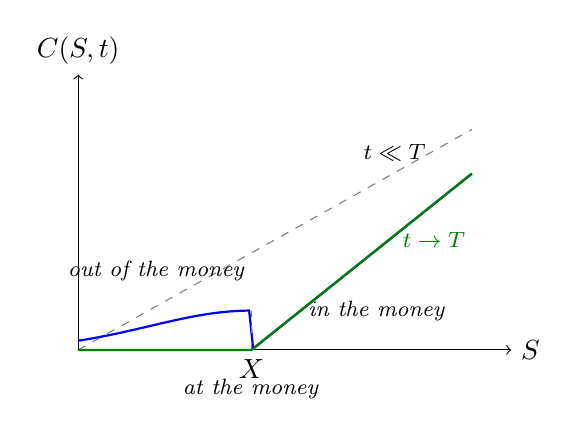
\begin{tikzpicture}
    \draw[->] (0,0) -- (5.5,0) node[right] {$S$};
    \draw[->] (0,0) -- (0,3.5) node[above] {$C(S,t)$};
    \draw[thick, blue, domain=0:5, samples=100]
        plot (\x, {max(0, \x - 2.2)*0.8 + 0.5*exp(-0.3*(2.2-\x)^2)*(\x < 2.2 ? 1 : 0)});
    \draw[dashed, gray] (0,0) -- (5,2.8);
    \draw[dashed, gray] (2.2,0) -- (2.2,0.5);
    \node[below] at (2.2,0) {$X$};
    \node[right, font=\footnotesize] at (3.5,2.5) {$t \ll T$};
    \draw[thick, green!50!black] (0,0) -- (2.2,0) -- (5,2.24);
    \node[right, font=\footnotesize, green!50!black] at (4,1.4) {$t \to T$};
    \node[font=\footnotesize] at (1,1) {\emph{out of the money}};
    \node[font=\footnotesize] at (3.8,0.5) {\emph{in the money}};
    \node[font=\footnotesize] at (2.2, -0.5) {\emph{at the money}};
\end{tikzpicture}
\caption{The Black--Scholes call value $C(S,t)$ before maturity (blue), smoothing the terminal hockey-stick payoff (green); as $t\to T$ the curve collapses onto the payoff.}
\label{fig:call-value}
\end{figure}

\subsection{The European put and put-call parity}

The same computation with the put payoff $\{X-S_T\}_+$ gives
\begin{equation}\label{eq:bs-put}
P(S,t) = X\, e^{-r(T-t)}\, N(-d_2) - S\, N(-d_1).
\end{equation}
(The great practical problem of both formulas, to which we return in Section~\ref{sec:volatility}, is the volatility of the underlying, which is not directly observable.)

Puts and calls are not independent instruments, however.
Subtracting the two formulas and using $N(-x)=1-N(x)$,
\begin{equation}
P(S,t) - C(S,t) = -S + X\, e^{-r(T-t)},
\end{equation}
or equivalently,
\begin{equation}\label{eq:put-call-parity}
P(S,t) = C(S,t) - S + X\, e^{-r(T-t)}.
\end{equation}
This is the \emph{put-call parity}: a deterministic, model-independent relation between the two prices.
It is a direct consequence of the no-arbitrage principle --- the portfolio ``long a call, short a put, short the stock'' has a deterministic payoff at maturity, and must therefore earn exactly $r$ --- and it holds regardless of the Black--Scholes hypotheses.
Any quoted pair of put and call prices violating~\eqref{eq:put-call-parity} is free money, and traders make sure it never lasts.


\section{The Greeks}\label{sec:greeks}

The Black--Scholes price is a function of many variables, and its partial derivatives --- universally known as \emph{the Greeks} --- measure the sensitivity of the option to each of them.
They are the risk-management dashboard of every derivatives desk.

\subsection{Delta}

The first and most important Greek is the hedge ratio itself,
\begin{equation}
\Delta_C(S,t) = \frac{\partial O(S,t)}{\partial S} = \frac{\partial C(S,t)}{\partial S},
\end{equation}
the quantity of stock the writer must hold at every instant.
Differentiating the call formula~\eqref{eq:bs-call},
\begin{equation}
\Delta_C(S,t) = N(d_1) + \biggl\{S\,\frac{\partial N(d_1)}{\partial d_1}\frac{\partial d_1}{\partial S} - X\, e^{-r(T-t)}\,\frac{\partial N(d_2)}{\partial d_2}\frac{\partial d_2}{\partial S}\biggr\}.
\end{equation}
The term in braces looks alive, but it is not: using $N'(d_i) = \frac{1}{\sqrt{2\pi}}\, e^{-d_i^2/2}$ together with the relation $d_1 = d_2 + \sigma\sqrt{T-t}$, a careful calculation shows that the two contributions cancel identically, leaving the remarkably clean result
\begin{equation}\label{eq:delta-call}
\Delta_C(S,t) = N(d_1).
\end{equation}
For the put, differentiating the parity relation~\eqref{eq:put-call-parity} term by term,
\begin{equation}\label{eq:delta-put}
\Delta_P(S,t) = -(1 - N(d_1)) = N(d_1) - 1.
\end{equation}
The function $N(d_1)$ is approximately a step function centred at $X$, but broadened by the volatility: deep out of the money the writer holds almost no stock, deep in the money almost the full share, and near the strike the hedge transitions smoothly.
Delta also gives the trader's rule of thumb for small price moves,
\begin{equation}
C(S+dS) \approx C(S) + \Delta\, dS.
\end{equation}

\subsection{Other Greeks}

In the model $r$ and $\sigma$ are constants; in reality they fluctuate, and their own sensitivities get names too:
\begin{align}
\rho &:= \frac{\partial O}{\partial r}, \\[3pt]
\Theta &:= -\frac{\partial O}{\partial t} \qquad (\text{with } \tau = T - t), \\[3pt]
\nu &:= \frac{\partial O}{\partial \sigma} \qquad (\text{vega}).
\end{align}
Rho measures exposure to interest-rate moves, Theta the inexorable decay of the option value as maturity approaches, and Vega --- the most watched of the three --- the exposure to changes in volatility.

\subsection{Interpretation of the writer's portfolio}

The Greeks make the writer's cash position interpretable.
For a \textbf{call}, substituting $\Delta_C = N(d_1)$,
\begin{equation}\begin{split}
\Pi(S,t) = C(S,t) - \Delta(S,t)\, S &= S\, N(d_1) - X\, e^{-r(T-t)} N(d_2) - N(d_1)\, S\\
&= -X\, e^{-r(T-t)}\, N(d_2).
\end{split}\end{equation}
Every factor now speaks: $X$ is the amount the holder will pay the writer at $T$ if the call is exercised; $e^{-r(T-t)}$ discounts that payment from maturity to the present; and $N(d_2)$ is the probability that the exercise actually happens.
The writer's debt is exactly the discounted, probability-weighted strike.
For a \textbf{put}, the same substitution gives
\begin{equation}\begin{split}
\Pi(S,t) = P(S,t) - \Delta_P(S,t)\, S &= X\, e^{-r(T-t)}\, N(-d_2) - S\,N(-d_1) + N(-d_1)\,S\\
&= X\, e^{-r(T-t)}\, N(-d_2),
\end{split}\end{equation}
with the mirror-image reading: $X$ is what the writer will receive from the holder, and $N(-d_2)$ is the probability of exercise of the put.


\section{Volatility}\label{sec:volatility}

The Black--Scholes price $C_{\text{BS}} = C_{\text{BS}}(S, t, X, T, r, \sigma)$ depends on six quantities.
Five of them are either written in the contract ($X$, $T$), read off the market ($S$, $t$), or proxied by government bonds ($r$).
The sixth, $\sigma$, is different: it is the most critical input and the only \emph{hidden} one --- no screen displays the volatility.
Estimating it is a subject in itself, and there are two philosophies.

\subsection{Historical volatility}

The first philosophy looks backwards: the \emph{historical} (or \emph{realized}) volatility is extracted from a statistical analysis of real time series.
The GBM model says that log-returns over a step $\Delta t$ satisfy
\begin{equation}
d\ln S(t) = \ln\frac{S(t+\Delta t)}{S(t)} = \mu^*\!\Delta t + \sigma\, dW_t, \qquad \mu^* = \mu - \frac{\sigma^2}{2},
\end{equation}
where the most common choice is daily returns ($\Delta t = 1$ day), although today one can go below the minute (\emph{high-frequency} data).
The relevant moments are
\begin{align}
\mathbb{E}\!\biggl[\ln\frac{S(t+\Delta t)}{S(t)}\biggr] &= \mu^*\!\Delta t, \\[4pt]
\mathrm{Var}\!\biggl[\ln\frac{S(t+\Delta t)}{S(t)}\biggr] &= \sigma^2\Delta t
\quad\Longrightarrow\quad
\sigma = \sqrt{\frac{1}{\Delta t}\,\mathrm{Var}\!\bigl[\cdots\bigr]},
\end{align}
where the first is the historical instantaneous return and the second yields the volatility, with the tell-tale dimension $[\sigma] = t^{-1/2}$ (typically days$^{-1/2}$).

Here, however, we run into the conceptual problem announced in Chapter~3.
The expectations above are \emph{ensemble} averages, over infinitely many copies of the market; what we possess is a single time series $S_k$, $k=0,\ldots,N-1$ --- \emph{one} realization (the same predicament as in meteorology).
Time averages equal ensemble averages only for stationary processes, and the market is \emph{not} stationary: both $\mu^*$ and $\sigma$ drift over the years.
Strictly speaking, then, the procedure is unjustified; but no better tool exists, so one proceeds anyway, with eyes open, using the sample estimators
\begin{align}
\mu^* &\;\longrightarrow\; m = \frac{1}{\Delta t}\,\frac{1}{N}\sum_{k=0}^{N-1}\ln\frac{S_{k+1}}{S_k}, \\[6pt]
\sigma^2 &\;\longrightarrow\; S^2 = \frac{1}{\Delta t}\,\frac{1}{N-1}\sum_{k=0}^{N-1}\Bigl(\ln\frac{S_{k+1}}{S_k} - m\Bigr)^{\!2}, \qquad S = \sqrt{S^2} = \sigma_{\text{historical}}.
\end{align}
Even then, judgement is required: there is no scientific criterion for the choice of the window $N$.
Traders often take one year of data --- go too far back and the market was a different, possibly turbulent, animal.
For greater accuracy one can use high-frequency returns, obtaining $\sigma_{\text{hf}}$.
In all cases $\sigma_{\text{hist}}$ depends critically on $\Delta t$ and $N$: two analysts with different windows will disagree.

\subsection{Implied volatility}

The second philosophy looks forwards, and inverts the logic.
Historical volatility summarizes the past; but options are being traded \emph{now}, at prices the market has already agreed on, and those prices embody the market's collective expectation of \emph{future} volatility.
The \emph{implied volatility} is defined by \emph{calibration}: it is the value $\sigma_{\text{implied}}$ that makes the model reproduce the market,
\begin{equation}
C_{\text{market}} = C_{\text{BS}}(S, t, X, T, r, \sigma_{\text{implied}}).
\end{equation}
The Black--Scholes formula cannot be inverted for $\sigma$ analytically, so one solves
\begin{equation}
C_m - C_{\text{BS}}(S, t, X, T, r, \sigma_{\text{implied}}) = 0
\end{equation}
numerically, by iteration (e.g.\ Newton's method) --- fast and routine.
Implied volatility is thus a market-quoted forecast, reflecting expectation rather than history.

\subsection{The volatility smile}\label{sec:volatility-smile}

Implied volatility also hands us a clean, self-contained test of the model.
If Black--Scholes were exactly right, options with different strikes $X$ on the same underlying would all imply the \emph{same} $\sigma$ --- the volatility is a property of the stock, not of the contract.
Plotting $\sigma_{\text{impl}}$ against $X$, the data disagree: one finds a roughly parabolic shape, lowest near the current price and rising on both wings, universally known as the \textbf{volatility smile} (Figure~\ref{fig:smile}).
% CLAUDE NOTE (unreviewed section): The notes contain a rough sketch of the smile.
% We provide a proper TikZ rendering and expanded explanation.

\begin{figure}[h!]
\centering
\begin{tikzpicture}
    \draw[->] (0,0) -- (5.5,0) node[right] {$X$};
    \draw[->] (0,0) -- (0,3.2) node[above] {$\sigma_{\text{impl}}$};
    \draw[thick, blue, domain=0.5:5, samples=80]
        plot (\x, {0.3*(\x-2.75)^2 + 1.0});
    \node[below] at (2.75,0) {$S$};
    \draw[dashed, gray] (2.75,0) -- (2.75,1.0);
\end{tikzpicture}
\caption{The volatility smile: implied volatility as a function of the strike $X$, minimal near the spot price $S$ and rising on the wings. A constant-$\sigma$ model would predict a horizontal line.}
\label{fig:smile}
\end{figure}

The smile is the market telling us that the constant-$\sigma$, Gaussian world of Black--Scholes underprices extreme events: buyers of far out-of-the-money options (bets on large moves) are willing to pay more than the Gaussian tail would justify, and the excess shows up as higher implied volatility.
The same message appears in the time series: with a truly constant $\sigma$, the log-returns $\ln(S_{k+1}/S_k)$ would look like a homogeneous random walk, whereas real returns display \emph{intermittency} --- bursts of high volatility separated by calm stretches, the volatility clustering already mentioned.
The conclusion is twofold: $\sigma$ is the quantity that must be watched most carefully, and the Black--Scholes model, while analytically wonderful, has identified its own critical weakness --- volatility.
% CLAUDE NOTE (unreviewed): The notes mention that once σ is identified as the critical
% quantity, B-S can be applied numerically to other option types as well.
Chapter~7 takes up the models that promote $\sigma$ to a stochastic process of its own.


\section{The CRR binomial model}\label{sec:crr}

The Black--Scholes formula covers European plain vanilla options; for anything more exotic --- and for American options in particular --- closed formulas rarely exist, and one needs a numerical method.
The most elegant one is the \emph{binomial tree} of Cox, Ross, and Rubinstein (1979)\cite{CRR1979}, the CRR model: a discretization of the GBM so natural that it doubles as an independent derivation of Black--Scholes.
% CLAUDE NOTE (unreviewed section): The notes from here to the end (pages 15–17) are
% unreviewed. The original notation and derivation are preserved in comments where they
% differ from the standard treatment; the main text follows the canonical formulation.

\subsection{The binomial tree}\label{sec:binomial-tree}

On the interval $[0, T]$, introduce a time step $\Delta t = T/N$ with $N\gg 1$ (in practice $\sim 10^5$), so that time becomes discrete.
The brutal simplification --- and the source of all the model's tractability --- is this: at each step, the stock price is allowed only \emph{two} moves,
\begin{equation}
S \;\longrightarrow\;
\begin{cases}
S_u = S\, u & \text{(up move), with probability } p, \\
S_d = S\, d & \text{(down move), with probability } 1-p,
\end{cases}
\qquad d < 1 < u.
\end{equation}
Three unknowns, then: $p$, $u$, and $d$.
Three conditions will pin them down, each with a clear meaning.

The first condition matches the \emph{mean}: after one step, the expected stock value must grow at the risk-neutral rate,
\begin{equation}\label{eq:crr-mean}
\mathbb{E}[S(\Delta t)] = p\, S_u + (1-p)\, S_d = p\, Su + (1-p)\, Sd = S\, e^{r\Delta t}.
\end{equation}

The second condition matches the \emph{variance}: the log-returns over one step must have the GBM variance,
\begin{equation}
\mathrm{Var}\!\biggl[\ln\frac{S(t+\Delta t)}{S(t)}\biggr] = \sigma^2\Delta t.
\end{equation}
Since $\frac{\Delta S}{S}\approx \ln\bigl(1+\frac{\Delta S}{S}\bigr)$ for $\Delta S \ll S$, we may work with the two-point distribution
\begin{equation}
\tilde P\Bigl(\frac{\tilde S}{S}\Bigr) = p\;\delta\Bigl(\frac{\tilde S}{S}-u\Bigr) + (1-p)\;\delta\Bigl(\frac{\tilde S}{S}-d\Bigr),
\end{equation}
whose variance is computed in two lines:
\begin{equation}\label{eq:crr-var}
\mathrm{Var}\!\Bigl[\frac{\Delta S}{S}\Bigr] = p\, u^2 + (1-p)\, d^2 - \bigl[p\, u + (1-p)\, d\bigr]^2 = p(1-p)(u-d)^2 = \sigma^2\Delta t.
\end{equation}

Equations~\eqref{eq:crr-mean} and~\eqref{eq:crr-var} are two conditions for three unknowns; the third is a choice of convenience, but a crucial one.
We require the tree to be \emph{recombining}:
\begin{equation}
u\, d = 1,
\end{equation}
meaning that an up move followed by a down move returns the price exactly to its starting value.
The payoff of this choice is combinatorial: without recombination the tree has $2^N$ distinct nodes after $N$ steps --- computationally hopeless --- whereas with it the branches merge (Figure~\ref{fig:binomial-tree}) and only $\sim N^2$ nodes survive.

\begin{figure}[h!]
\centering
\begin{tikzpicture}[scale=1.1]
    \node (S) at (0,0) {$S$};
    \node (Su) at (2,1) {$Su$};
    \node (Sd) at (2,-1) {$Sd$};
    \node (Suu) at (4,2) {$Su^2$};
    \node (Sud) at (4,0) {$S$};
    \node (Sdd) at (4,-2) {$Sd^2$};
    \draw[->] (S) -- (Su) node[midway, above left, font=\footnotesize] {$p$};
    \draw[->] (S) -- (Sd) node[midway, below left, font=\footnotesize] {$1-p$};
    \draw[->] (Su) -- (Suu);
    \draw[->] (Su) -- (Sud);
    \draw[->] (Sd) -- (Sud);
    \draw[->] (Sd) -- (Sdd);
\end{tikzpicture}
\caption{The first two steps of a recombining binomial tree ($ud=1$): the up-down and down-up paths land on the same node, keeping the number of nodes quadratic rather than exponential in the number of steps.}
\label{fig:binomial-tree}
\end{figure}

Solving the system: from~\eqref{eq:crr-mean},
\begin{equation}\label{eq:crr-p}
p = \frac{e^{r\Delta t} - d}{u - d},
\end{equation}
and the jump sizes are
\begin{equation}\label{eq:crr-ud}
u = e^{\sigma\sqrt{\Delta t}}, \qquad d = e^{-\sigma\sqrt{\Delta t}}.
\end{equation}
These are approximate solutions, correct to leading order: expanding $e^{r\Delta t}(u+d) - ud - e^{2r\Delta t}$ in powers of $\Delta t$ reproduces $\sigma^2\Delta t$, as the variance condition requires.
Note the $\sqrt{\Delta t}$ in the exponents --- the diffusive scaling of Chapter~3, resurfacing in discrete time.

The bookkeeping of the tree is handled by two indices: the time index $i=0,\ldots,N$ and the up-move count $j=0,\ldots,i$, in terms of which the stock price at node $(i,j)$ is
\begin{equation}\label{eq:crr-price}
S_{i,j} = S\, u^j\, d^{i-j}.
\end{equation}

\subsection{Option pricing on the binomial tree}\label{sec:crr-pricing}

To price an option on the tree, we replay the Black--Scholes hedging argument in discrete time.
The trader's wealth is $W = \Pi + \Delta S = C$, where $C=C(0)=C(S(0))$ and $\Pi=\Pi(0)$; a price move $dS$ induces $dC$ and $d\Pi$, with $\Delta = \partial C/\partial S$ playing its usual role.
Over one step the world splits in two: if $S$ goes up, $C\to C_u$ and $\Pi\to\Pi_u$; if down, $C\to C_d$ and $\Pi\to\Pi_d$.
Risk neutrality of the hedged portfolio demands $\Delta\Pi = \Pi_u - \Pi_d = 0$, i.e.
\begin{equation}
C_u - \Delta S_u = C_d - \Delta S_d \quad\Longrightarrow\quad
\Delta_{\text{CRR}} = \frac{C_u - C_d}{S_u - S_d},
\end{equation}
the discrete difference quotient replacing the derivative $\partial C/\partial S$ --- delta hedging without calculus.
The riskless portfolio must then earn the risk-free rate, $\Pi\, e^{r\Delta t} = (C - \Delta S)\, e^{r\Delta t}$, which holds precisely when $\Delta = \Delta_{\text{CRR}}$; substituting and simplifying,
\begin{equation}\label{eq:crr-option}
C_{\text{CRR}} = e^{-r\Delta t}\bigl\{p\, C_u + (1-p)\, C_d\bigr\}.
\end{equation}
Pause on the structure of this result: the option price today is the \emph{discounted expectation of tomorrow's prices under the probability $p$} --- and $p$, from~\eqref{eq:crr-p}, is not the real-world probability of an up move but the risk-neutral one, built from $r$.
Equation~\eqref{eq:crr-option} is the Feynman--Kac formula~\eqref{eq:feynman-kac-discount} in its simplest possible incarnation: one step, two states.

\subsection{The backward algorithm}\label{sec:crr-algorithm}

Iterating~\eqref{eq:crr-option} from maturity back to the present prices the option; the recipe is called \emph{backward induction}.
For a European plain vanilla call it reads:

\begin{enumerate}[label=\alph*)]
    \item \textbf{Initialize:} given $X$ and $S$, set $T=1$, $N$, and $\Delta t = T/N$.
    Given $r$ and $\sigma_{\text{implied}}$, compute $p$, $1-p$, $u$, $d$ from \eqref{eq:crr-p} and \eqref{eq:crr-ud}.

    \item \textbf{Forward sweep} (build the tree):
    for $i=1,\ldots,N$ and $j=0,\ldots,i$, compute
    \begin{equation}
    S_{i,j} = S\, u^j\, d^{i-j}.
    \end{equation}

    \item \textbf{Terminal payoff:}
    at maturity ($i=N$), for $j=0,1,\ldots,N$, set
    \begin{equation}
    C_{N,j} = \max\{S_{N,j} - X,\; 0\}.
    \end{equation}

    \item \textbf{Backward sweep} (price the option):
    for $i=N-1,\ldots,0$ and $j=0,\ldots,i$, apply
    \begin{equation}
    C_{i,j} = e^{-r\Delta t}\bigl\{p\, C_{i+1,\,j+1} + (1-p)\, C_{i+1,\,j}\bigr\}.
    \end{equation}
    The option price is $C_{0,0}$.
\end{enumerate}

A miniature example makes the mechanics concrete.
With $N=3$, the terminal layer $i=3$ has four payoffs $C_{3,0},\ldots,C_{3,3}$; the layer $i=2$ combines them pairwise into three values $C_{2,j} = e^{-r\Delta t}\{p\, C_{3,j+1} + (1-p)\, C_{3,j}\}$; the layer $i=1$ gives two; and the root $i=0$ delivers the fair price $C_{0,0}$.\footnote{The convergence $C_{\text{CRR}} \to C_{\text{BS}}$ as $N\to\infty$ is guaranteed by the central limit theorem: the binomial distribution of the terminal node converges to the Gaussian, and the discrete-time model recovers the continuous-time GBM.}

\subsection{Extensions}\label{sec:crr-extensions}

The real payoff of the binomial framework is how little needs changing to price non-standard contracts; two examples close the chapter.

\subsubsection{Barrier options}

A \emph{barrier option} (of knock-out type) dies if the stock price ever crosses a barrier $U$ during the life of the contract.
On the tree, this is a one-line modification of the backward sweep: at every node,
\begin{equation}
\forall\, i,j: \quad
\begin{cases}
S_{i,j} > U &\Longrightarrow\; C_{i,j} = 0, \\
S_{i,j} \le U &\Longrightarrow\; C_{i,j} = e^{-r\Delta t}\bigl\{p\, C_{i+1,j+1} + (1-p)\, C_{i+1,j}\bigr\},
\end{cases}
\end{equation}
i.e.\ the barrier condition is simply imposed node by node.\footnote{For knock-\emph{in} barrier options the logic is reversed: the option only comes alive once the barrier is crossed.}

\subsubsection{American options}

For an \emph{American} option, the holder may exercise at any time $t\le T$, and the tree handles this with equal ease.
At each node $(i,j)$ the holder faces a choice --- exercise now, or hold on --- and rationality dictates taking the better of the two:
\begin{equation}\label{eq:american-option}
C^A_{i,j} = \max\!\bigl\{S_{i,j} - X,\; e^{-r\Delta t}[p\, C^A_{i+1,j+1} + (1-p)\, C^A_{i+1,j}]\bigr\},
\end{equation}
the maximum of the \emph{exercise value} and the \emph{continuation value} (the discounted no-arbitrage value of keeping the option alive).
When $S_{i,j} < X$ the exercise value is nil and the American option behaves like a European one; when $S_{i,j} > X$ early exercise may become optimal, capturing $S_{i,j}-X$ immediately rather than waiting.\footnote{For American \emph{calls} on non-dividend-paying stocks, one can show that the continuation value always exceeds the exercise value, so early exercise is never optimal and the American call equals the European one. For American \emph{puts}, by contrast, early exercise can be genuinely optimal.}

With options priced --- analytically when we can, numerically when we must --- we turn in the next chapter to the other great family of financial instruments: bonds, and the stochastic dynamics of interest rates that governs them.
